\chapter{Basics of Linux kernel} %Capitolo in comune
\label{ch:introduction}

\section{Operating Systems}
\label{sec:os}
The operating system (OS) comprises the software intended to manage the hardware resources and the \textit{application software}, which performs specific, high-level tasks. The application software, which is the larger part of the OS, is made of utility programs and any other software with which the user interacts directly. These programs are not part of the core OS. Rather, they are necessary to do anything useful. The operating system acts as an intermediary between the user and the machine by abstracting away the hardware, which makes interaction easier: this is why almost every computer runs an operating system.

It can be argued that the OS is not strictly necessary because it's possible to execute a program without loading an OS: this is referred as \textit{bare metal programming} which is common in small size embedded systems. Because there is no operating system (which means no file system, memory management or any useful application such as compilers), programs cannot be written on the system itself. Instead, the program is written on another machine with an operating system, then compiled with a cross-compiler, which compiles for a target architecture different from the one it is running on. Finally, the compiled binaries are loaded at boot time on the target embedded system. This is the opposite of what we are used to do on our laptops/desktops: to be able to reprogram the machine as it is running, by writing and compiling our program with \textit{application software} designed to edit text and compile code. Thus, an operating system greatly simplifies interaction with the machine by offering a platform for the user and, at a higher level, by making general-purpose computing possible.
%There are also OSes for embedded systems called \textit{real-time systems}, but we will focus only on general-purpose OSes. 

Windows, MacOS, iOS, Android\dots\   Most of us are familiar with these operating systems. Besides the platform on which they run, they are all general-purpose and their goal is the same. What really changes among them is the architecture and philosophy in their design. At a macroscopic level they differ in kernel design approach (monolithic kernel vs.\ hybrid kernel). This is explained later in section \ref{img:monolithic}. At a microscopic level, there is literally not much to see because the code of most OSes is closed, so it's impossible to see the implementation differences with Linux. This leads us to one of the peculiarities of Linux: it's completely open source and community developed. Besides ethical matters, which are not discussed here, this means that it's possible to study the code and get a full understanding of operating systems. In fact, before Linux, there was no way to see how operating systems work in practice. The only option was to study them from textbooks in order to implement your own kernel, which is exactly what Linus Torvalds did.

As stated earlier, a key component of an OS is ``the software intended to manage the hardware resources'': this is what we refer as the \textit{kernel}. Dennis Ritchie, among the inventors of Unix and C, also called it the ``Operating system proper''\cite{ritchie}, which most likely means ``The component that is the actual operating system''. On the one hand this definition makes sense, because the low level tasks performed by the kernel are essential (and also because it's the most difficult component to develop). But on the other, without application software the kernel is useless. In such scenario, the kernel is loaded at boot, then it initializes and starts running, and then there is nothing but a black screen because there is no other program to start. It's clear that the kernel is not an operating system by itself, but what Dennis meant is that when we think about the core architecture of an OS, we think about the kernel. An engine is indeed useless without the rest of the car, but does that make the other components as important as the engine, where all the complexity resides? Despite the application software being the largest part of the OS; it is within the kernel that the hardest engineering challenges are found, which makes it the most interesting---and difficult---part to understand and analyze.

\section{A general overview} 
\label{sec:general}
The kernel's job is to manage hardware resources, which means handling all interactions with the CPUs, the memory hierarchy and the I/O devices. More specifically, the kernel needs to respond to I/O requests, manage memory allocation and decide how the CPU time is shared among the demanding processes. To achieve this, it has access to all resources in the system, which is needed to make the most out of the hardware. Its performance is what makes the difference between a fast or a slow operating system. This critical role requires a protection mechanism to ensure the stability and the security of the whole system. This is achieved by separating kernel code and user application code. In practice, depending on the configuration settings at compile time, what happens is: 
\begin{enumerate}
    \item The kernel binary image is loaded in RAM in a memory area which can start from a low or high address.
    \item A predefined slice of RAM next to that memory area is reserved to the kernel. 
    \item The remaining part of the memory is accessible to the user.
\end{enumerate}
These two portions of the address space %of RAM
are called kernel space and user space. The former is a reserved area dedicated to critical system tasks and it's protected from user access, the latter is the area where system utilities and user programs run. This memory partitioning makes sure that kernel and user data do not interfere with each other. Also, it is a security measure to prevent that a malfunctioning or malicious user program may affect the entire system.

\subsection{System calls}
By extension of this design, the interaction with the user space is regulated with a privilege system. Each process can run either in user mode or kernel mode. Processes running in user mode can access privileged kernel functionalities through special gates in a predefined and controlled manner. These gates are implemented as functions called \textit{system calls}, which serve as APIs between user and kernel space. When a user process performs a system call
\begin{enumerate}
    \item it temporarily executes in kernel mode, 
    \item it performs tasks that require a high privilege, and finally
    \item it switches back to low privilege.
\end{enumerate}
This mechanism exploits the availability of hardware functionalities.
For example, in the x86 architecture 2 bits in the code selector (\verb|cs|) register indicate the current privilege level (CPL) of the program that is running on the CPU. This value is 0 or 3, respectively, for kernel and user mode and each system call changes this value temporarily. 

\begin{figure}[ht]
  \centering
  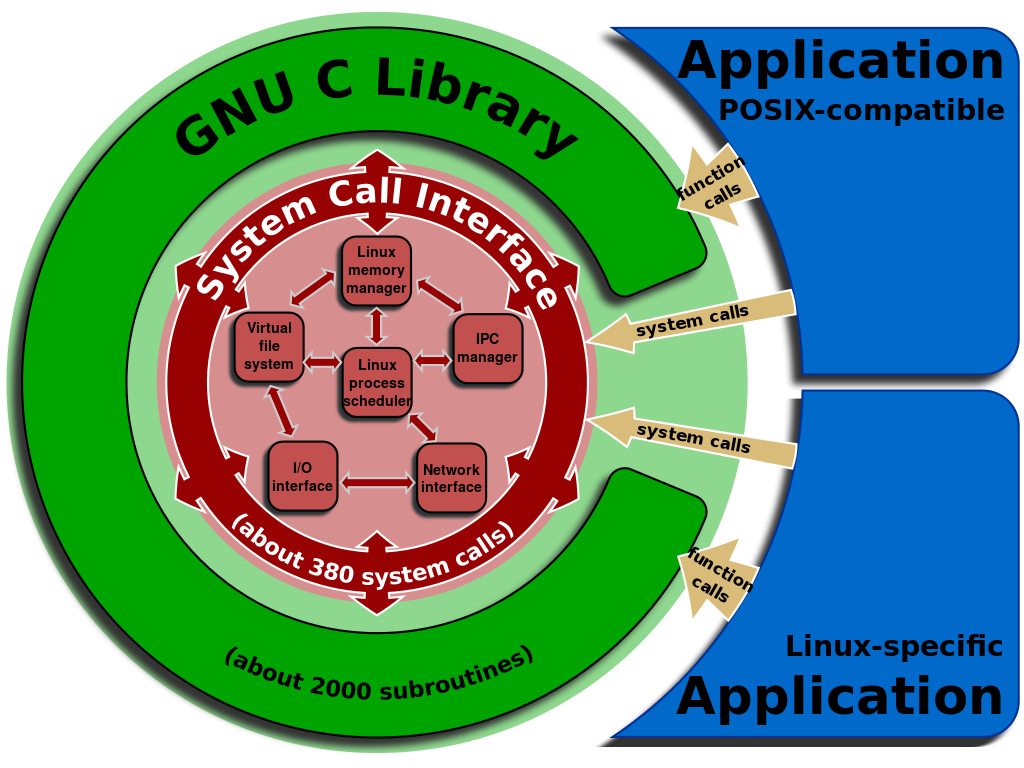
\includegraphics[width=.75\textwidth]{images/userspace_kernelspace.png}
  \caption{Kernel space (in red) and user space (in green and blue)}
  \label{img:userspace_kernelspace}
\end{figure}

Very often, useful operations in the system require privileged services provided by the kernel. For example, even an extremely simple shell command such as \verb|echo| performs dozens of system calls, which are reported below as listed by the command \verb|strace -wc echo|
\begin{Verbatim}
% time     seconds  usecs/call     calls    errors syscall
------ ----------- ----------- --------- --------- ----------------
 29.57    0.000514         514         1           execve
 17.03    0.000296          33         9           mmap
 11.62    0.000202          67         3           brk
  8.52    0.000148          37         4           mprotect
  7.19    0.000125          25         5           close
  6.10    0.000106          35         3           open
  5.93    0.000103          26         4           fstat
  5.58    0.000097          32         3         3 access
  2.82    0.000049          49         1           munmap
  2.24    0.000039          39         1           write
  1.84    0.000032          32         1           read
  1.55    0.000027          27         1           arch_prctl
------ ----------- ----------- --------- --------- ----------------
100.00    0.001738                    36         3 total
\end{Verbatim}
System calls can be called in user space applications directly, through assembly, or indirectly, by calling wrapper functions from the C standard library (\verb|glibc|), as shown in Figure\ref{img:userspace_kernelspace}. 
\begin{code}
// Two different ways of calling open/close through glibc wrapper functions 
// SYS_open and SYS_close correspond o the syscall numbers
int fd = syscall(SYS_open, "example.txt", O_WRONLY);
syscall(SYS_close, fd);
fd = open("example.txt", O_WRONLY);
close(fd);
\end{code}
Calling through assembly means filling the right CPU register with the syscall arguments and then using a special assembly instruction. On x86 machines it is required to fill the \verb|EAX| register with the system call number (by a \verb|mov| assembly instruction) and then invoke the interrupt 128 (by the instruction \verb|int 0x80|). Modern processors may use a different one. This is what will happen upon its execution:
\begin{enumerate}
    \item Interrupt number 128 (=\verb|0x80|) is released. In Linux, it corresponds to a system call interrupt. 
    \item The process execution is suspended and the control passes to the kernel (kernel mode), which will look up the entry 128 in the \textit{interrupt vector table}. This table simply associates interrupt numbers with their handler: a function that gets executed when the interrupt happens.
    \item The corresponding handler is executed: this function copies the syscall number and arguments from the registers onto the kernel stack. It will then look up in the \textit{system call dispatch table} the handler corresponding to the syscall number and call it with the correct arguments like any normal C function, because the arguments are now located on the kernel stack.
    \item The system call is finally executed and the return value is stored in a general purpose data register.
\end{enumerate}
Registers are used to pass the parameters because this way it's easier to get them from user to kernel space. It is intuitive that such a procedure to invoke system calls is architecture dependent. For this reason, \verb|glibc| wrappers are always used: they internally execute the assembly code that we just illustrated and do it differently for each architecture.
%(you can write assembly into C source code, more on this later).
Calling wrappers is also very safe since it avoids to accidentally fill the wrong registers or miss the right number of arguments.
%and, moreover, most syscalls have a wrapper so there's no reason to write assembly for them.
It's important to note that the kernel can protect itself against invalid syscall arguments in registers. This is crucial since, as we saw, syscalls are easily called from user space directly by executing the proper assembly instructions.

\subsection{A different kind of software}
The separation between kernel/user space and the fact that we are working at such low level makes the kernel a very peculiar piece of software. One of its properties is that there is no error checking, this is because the kernel trusts itself: all kernel functions are assumed to be error-free, so the kernel does not need to insert any protection against programming errors\cite{cesati}. Instead, what the kernel does is to use assertions to check hardware and software consistency; if they fail then the system goes into \textit{kernel panic} and halts. Later on in Section \ref{ch:events_documentation}, it is shown an example of code where the \verb|panic()| routine is called. The choice of checking assertion (and possibly going to kernel panic is something went wrong) is that since the kernel controls the system itself, error recovery and error correction is very hard and would take a huge part of the code. Another way of thinking about it, is that there is no meta-kernel that handles kernel errors. Of course programming or hardware errors can (and will) still occur: when this happens the offending process is killed and a memory dump called ``\textit{oops}'' is created. A typical example of this is when the kernel dereferences a NULL pointer: in user space this would cause a \textit{segmentation fault}, while in the kernel it will generate an oops or in the worst case go directly into panic. After this kind of event, the kernel can no longer be trusted and the best thing to do would be to reboot, because the kernel is in a semi-usable state and it could potentially corrupt memory. Furthermore, a panic in this state is more likely to happen. %oops count after the first one?
Possibly, the user experiencing the kernel panic may also inform the kernel mantainers.

% Ricordare di mettere parentesi quando si citano funzioni
Another peculiarity of the kernel is that it uses its own implementation of the functions in the standard C library. For example \verb|printf()| and \verb|malloc()| are implemented as \verb|printk()| and \verb|kmalloc()|. There are different reasons for this choice, one of those is that the C standard library is too big and inefficient for the kernel. Another reason is that implementing your own functions gives more freedom because they can be customized for their purpose in the kernel. Memory allocation in user or kernel space is very different, so the \verb|kmalloc()| implementation is very specific. For instance, kernel data structures need a contiguous physical memory segment to be allocated, while regular user space allocation doesn't have this restriction. Furthermore, \verb|printk()| writes its output into the kernel log buffer (that you can read by using the \verb|dmesg| command in user space); this is very different from \verb|printf()| that writes on standard output.

\subsection{User and kernel stacks}
As stated earlier, the memory management is different in kernel/user space.
The same applies to the execution. Every process in the system has two stacks, located respectively in user and kernel space, and it will use one of the two while executing in the corresponding privilege mode. x86 CPUs automatically switch stack pointers when privilege mode switches occur, which usually happens for syscalls. The user space stack can potentially be very big, with a very high limit (8MB on my machine, but it can be increased), and even though it's initially small it can allocate more physical memory as it needs it: this mechanism is called ``on-demand paging''. The kernel stack, unlike the user stack, cannot expand itself and it has a fixed size of two pages. Since, 32-bit and 64-bit systems have 4KB and 8KB sized pages, then the kernel stack size is of size 8KB or 16KB, respectively. These two pages must be allocated contiguously, which can cause memory fragmentation for long system uptimes as stacks get deallocated. In other words, it becomes increasingly hard to find two physically contiguous unallocated pages as the OS runs for a long time. For this reason, in the past efforts were made to reduce the stack size to one page, which would eliminate fragmentation, but after many stack overflows the standard settled on two pages.

This leads us to an interesting example of the kernel trusting itself: it makes the strong assumption that the stack will never overflow: \textbf{no protection against it is in place}. So what happens if it overflows? First, it will corrupt the \verb|thread_info| data structure, which is the first data that the stack encounters along its path (Figure \ref{img:stack}). This will make the process nonexistent for the kernel and cause a memory leak (we will see why). Next, the stack can overflow outside of the address space and silently corrupt whatever kernel data is stored; the best case scenario here would be a kernel panic to prevent any further memory corruption. Another natural question might be ``why are kernel stacks so small?'' and the answer is simple: first, to use a small amount of kernel memory, and secondly, because of fragmentation. The bigger is your data structure in contiguous physical memory, the more it is hard to allocate. It is expected that any process stays in kernel mode for a small amount of time, so it should use a very small portion of the stack. A consequence of small stacks is that very few recursive functions are used to avoid long call chains and minimize stack usage; the same is true for big static allocations on the stack. %check this

\begin{figure}[ht]
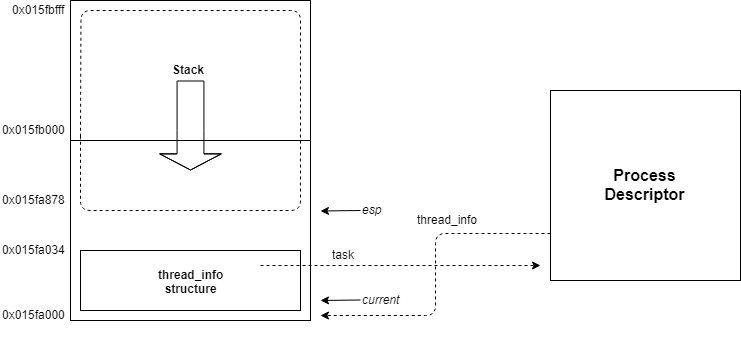
\includegraphics[width=\textwidth]{images/stack}
\caption{The kernel stack inside its small address space of two pages, it grows downward towards low memory.}
\label{img:stack}
\end{figure}

It's important to note that there are special processes called \textit{kernel threads} that do not follow this pattern of kernel/user stack. Kernel threads perform a specific system task, they are created by the kernel and they live exclusively in kernel space, never switching to user mode. Their address space is the whole kernel space and they can use it however they want. Besides this, they are normal and fully schedulable tasks just like the others. An example of a kernel thread is \verb|ksoftirqd|: there is always one for each CPU and their job is to dispatch interrupt requests. As a side note, the name stands for ``Kernel Software Interrupt ReQuest Daemon'', many kernel threads follow a similar naming convention. 
%Maybe mention per-CPU interrupt stacks? (for interrupt handlers)
%Interrupt stacks - To rectify this problem, the kernel developers implemented a new feature: interrupt stacks. Interrupt stacks provide a single per-processor stack used for interrupt handlers. With this option, interrupt handlers no longer share the kernel stack of the interrupted process. Instead, they use their own stacks. This consumes only a single page per processor.

\subsection{A monolithic design}
\label{sec:monolithic}
There are fundamentally different design approaches in kernel development. We can see these as a spectrum, where on one end there is the \textit{monolithic kernel}, and on the other one the \textit{microkernel} (or $\mu kernel$). The choice depends on how many services are located in kernel space: while in monolithic design every service is in the kernel itself, microkernels strive to reduce as much as possible the code running in kernel space. This is done by moving most services in user space, while keeping only essential primitives in the kernel (Figure \ref{img:monolithic}).

\begin{figure}[ht]
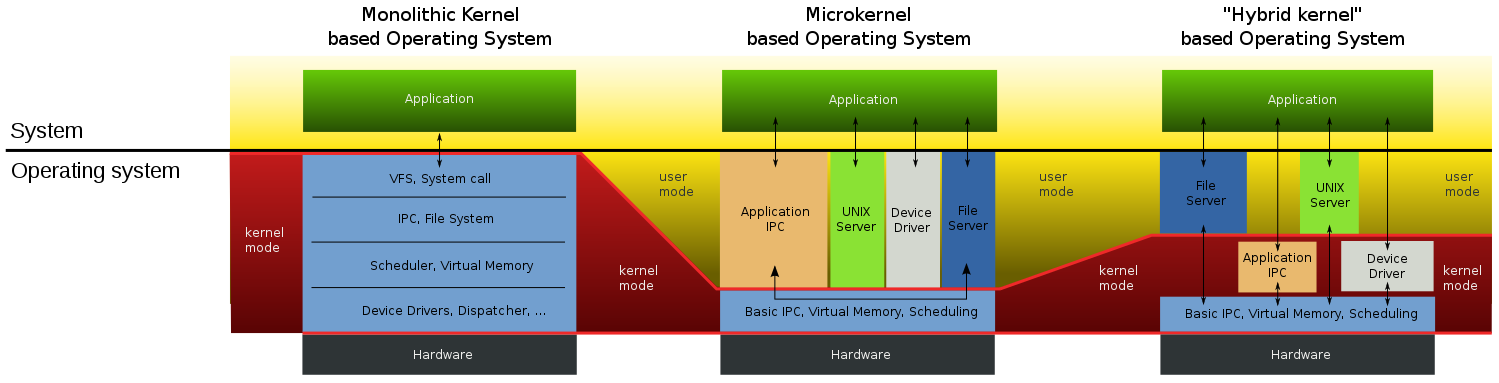
\includegraphics[width=\textwidth, keepaspectratio]{images/monolithic.png}
\caption{The most popular kernel designs and their differences}
\label{img:monolithic}
\end{figure}

These services are implemented as \textit{servers}, and communication between the servers, applications, and the kernel is based on message passing. As in classic client/server approach, applications send requests to the servers, which can in turn request services to the kernel or satisfy the request directly. Because of this design choice, the system relies heavily on \textit{Inter-Process Communication} (IPC), which can be achieved in different ways: in this case, there are actual messages being passed between processes. Even if they are part of the core architecture, the servers are user processes and run in user space just like the other user processes, though they get higher privileges.

By reducing the code running in kernel space, there is less risk for bugs. Because the trusted codebase is very small, there is no need to make big assumptions like in monolithic kernels. As stated before, a bug in the kernel can bring down the entire system, but in microkernels bugs are contained. For example, if the networking service crashes, then we can just restart it since it's just a user process; in a monolithic environnement, this problem would have crashed the entire system: this is one of the biggest flaws of the monolithic design. A small trusted codebase also means more portability because all the achitecture dependent code is concentrated in the small kernel. The actual operating system is built on top of it, so it would be possible to implement it in a more high level language, while only the primitives in the kernel must be ported. Conversely, in a monolithic kernel, many functions must be rewritten for each architecture: in Linux, the folder for architecture dependent code (\verb|arch|) is the second biggest folder and it represents 8\% of the code.

Another direct consequence of the shift of the code in user space is that microkernels are more easily maintainable. Development is easier because most of the code runs in user space, so the usual restrictions for kernel code are not present: for example, it would be possible to make use of \verb|glibc|. Furthermore, testing can be done without rebooting the system: just stop the service, recompile the code and then start it again. On a monolithic system, not only it's needed to recompile the whole kernel, we must also reboot in order to load the image again. And if this new image doesn't work, then we must reboot again with the working image. In practice, this is always done in a virtual machine in order to test more efficiently, but it's still a tedious process.

Given all these advantages, why aren't microkernels always used? It's (mostly) because of one deadly flaw: the performance penalty. It's easy to see this if we think that monolithic kernels communicate directly with hardware, while in microkernels most of the operating system does not; essentially, microkernels add an additional layer of abstraction though heavy use of IPC. More precisely, the task of moving in and out of the kernel to move data between the applications and servers creates significant overhead. This process results in two major problems:
\begin{itemize}
\item A large number of system calls, caused by services frequently needing to use the primitives.
\item Many context switches, because each service must be scheduled as a process. In order to pass a message between two services, a full context switch is needed to send and receive.
\end{itemize}
This last problem is not an issue in a monolithic setting, because kernel functions are executed when any currently running process enters kernel space. Of course, calling a plain function is much less costly than doing a system call or context switch. Furthermore, IPC in monolithic kernels is implemented through shared memory, which is more efficient than IPC with message passing. In Linux, because every functionality is in the kernel, it is a single, big program running in his dedicated address space: this means that every subsystem (scheduling, IPC, networking, memory management\dots) shares the same memory. Paradoxically, all the auxiliary code needed for interfacing and communication often makes microkernel-based operating systems larger than monolithic kernels, even though all this code is not in kernel space. 

Linux is a monolithic kernel, and because of this design choice, even the device drivers are located in kernel space: in fact, more than 65\% of the kernel code is just drivers (in the \verb|driver| directory, the largest folder). This means that while the system is running a huge part of the code is not being used. For this reason, many miniaturized versions of Linux have been distributed: a fully functional---and still monolithic---kernel can fit on a single floppy disk. If we wanted to create just a reduced version, it would not be too hard to remove drivers that are not needed and then recompile the kernel. 

A problem of the monolithic design is the natural lack of modularity; microkernels don't have this problem because it's very easy to start/stop drivers running in user space. Monolithic kernels try to achieve the modularity of microkernels by using \textit{kernel modules}: they are simply code that can be inserted/removed from the kernel at runtime. A module can be linked to the running kernel when its functionality is required and unlinked when it is no longer useful: this is quite useful for small embedded systems, to keep running code to a minimum. Modules are often used to add/remove drivers and this approach is much faster than having drivers in user space: since the code runs in kernel space, there is no need to do message passing or communicate with user space at all. It's just like in a microkernel and without performance penalty, but then again, now we are programming in kernel space, which is harder. In the end, it's a choice between ease of development/fault tolerance or performance. Furthermore, modules, unlike the external layers of microkernel operating systems, do not run as a specific process. Instead, they are executed in kernel mode on behalf of the current process, like any other kernel function: this means less switching between processes, so again, better performance. Because of the big flaw of monolithic kernels mentioned earlier, if a driver module doesn't behave correctly, the system can crash upon module insertion. In section \ref{sec:module} it's shown just how easy it is to crash the system by inserting our own---volountarily bugged---module. Needless to say, this operation requires root privileges: module insertion essentially means injecting arbitrary code in the kernel.

Modules are powerful, but cannot always accomplish what a microkernel can. As an example: on Linux, it's not possible to replace the scheduler at runtime. In order to do that, it's needed to have the two different schedulers directly in the core code and switch between them at runtime (This is how it's actually done in Linux: there are different schedulers already implemented). Modules usually aren't used to implement core functions, but are rather seen as extensions of the kernel. This means that is very difficult to modify policies decided by the kernel through modules, and users must adapt to these policies or modify the code and recompile the whole kernel. Conversely, in microkernels it's easy to change core implementation, since it runs as a service.

Finally, the hybrid design is halfway between monolithic and microkernel, as it tries to take the best side of both approaches: having good performance, but also, to some extent, flexibility and maintainability. In practice, its philosophy is very similar to a monolithic kernel and hybrid kernels have been dismissed by Linus Torvalds as ``just marketing''\cite{torvalds}. Notable OSes that use a hybrid kernel are Windows and MacOS.

\section{Process management}
The kernel is divided into subsystems that interact with each other. Figure \ref{img:kernelmap} is a zoom into the kernel mechanisms inside the red part of Figure \ref{img:userspace_kernelspace}. The image represents the part of the kernel that will be covered, for the most part we will swing between the scheduling and memory mapping subsystems. The names in the picture are structs, functions or source code files; we will get familiar with most of these as we go on.

\begin{figure}[t]
\centering
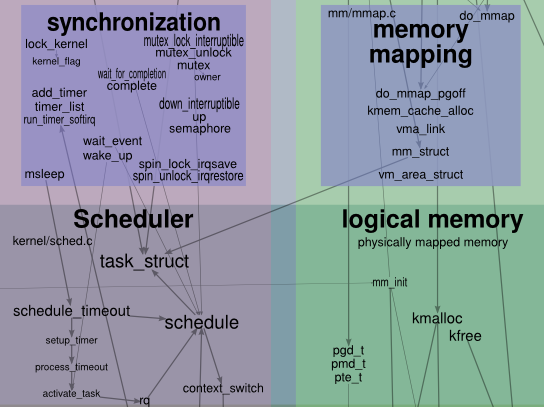
\includegraphics[width=0.9\textwidth]{images/kernelmap.png}
\caption{A portion of the kernel subsystems map (source: \url{www.google.com})}
\label{img:kernelmap}
\end{figure}

\subsection{Processes and threads}
\label{sec:proc_threads}
A process is an instance of a running program. Each process has resources associated with it, such as an address space, open files, global variables and code. Each process must have its own address space that only he can access: when a process tries to access a memory location that does not belong to it, a segmentation fault interrupt is generated. A thread is defined as a single flow of execution, it has associated a stack of execution and the set of CPU registers that it uses, most notably the stack pointer and program counter. Each process can have multiple threads, in which case it's a \textit{multi-threaded process}; threads belonging to a process will share resources between each other. The execution aspect of a process is always represented by threads, which means that a process cannot exist without at least one thread associated.

The kernel does not distinguish between processes and threads, so they are treated as the same entity. Because of this, a problem in terminology arises. Next, it is shown how processes ans threads are distinguished.

Each process has its own PID (Process IDentifier) and groups of processes are identified by the TGID (Thread Group ID). If a process has only a single thread then its PID is equal to its TGID. If a process is multi-threaded then each \textit{thread} has a different PID, but they will all have the same TGID. Furthermore, there will be a thread in this group called \textit{thread group leader} that will have its PID equal to the TGID, so the TGID field in each thread is just the PID of their leader. Just to add some more confusion, when you call \verb|getpid()| you are actually getting the TGID (the group leader PID, identifying the whole process), and when you call \verb|gettid()| you are getting the PID (which identifies a single thread, not a group). Hence, the PID resambles more a thread identifier.
%, that is also used as a process identifier when you have many threads associated to a process.
This confusing way of using IDs was implemented to comply with POSIX standards, which require that each thread of a multi-threaded process must have the same id: this is why \verb|getpid()| returns the TGID.

%You can already see how ``process'' and ``thread'' are being used interchangeably. As anticipated, this terminology can be confusing so let's clarify.
The real difference between threads and processes is that threads share the same address space, while processes do not. By saying that some threads are associated to a same process just means that they are sharing an address space. This enables concurrent programming, enables communication among threads via shared memory, and requires then synchronization methods. As shown in Section \ref{sec:scheduling},
using threads in a program instead of spawning new processes results in much better performance, which is why threads are sometimes called \textit{lightweight processes} or LWP.
\begin{code}
//stack size for cloned child
const int STACK_SIZE = 65536;
//start and end of stack buffer area
char *stack, *stackTop;
// ... define child startup function "do_something" ...
stack = malloc(STACK_SIZE);
stackTop = stack + STACK_SIZE; //stack grows downward

//spawns a new thread
clone(&do_something, stack + STACK_SIZE, CLONE_VM | CLONE_FS | CLONE_FILES | CLONE_SIGHAND, 0); 
//spawns a new process, this is the same as using fork()
clone(&do_something, stack + STACK_SIZE, SIGCHLD, 0); 
\end{code}
The system call \verb|clone()| spawns a new child process. It's very
similar to \verb|fork()| but it's more versatile because flags can be
used to decide how many resources are shared with the new
process. \verb|CLONE_VM| (where vm stands for virtual memory) makes
the child process run in the same address space as the father, while
the other flags clone filesystem information (such as working
directory), open files and signal handlers. The flag \verb|SIGCHLD| at
line 4 requires that the parent process receives a \texttt{SIGCHLD}
signal upon the termination of the created child process.  Ultimately,
the reason why threads and processes are treated as the same entity in
Linux, is that processes are just threads that share nothing. In fact,
the word \textit{task} is always used inside the kernel instead of
process/thread and we will do the same, especially when discussing
implementation.

Each task is represented in the kernel with the struct \verb|task_struct|, this is a fairly big structure that can be almost 2KB in size, depending on configuration at compile time. \verb|task_struct| is what is often referred as the \textit{process descriptor} or PCB (\textit{process control block}): every information about a task is stored in here. 
\begin{code}
struct task_struct {
	/* -1 unrunnable, 0 runnable, >0 stopped: */
	volatile long			state;
	void				*stack;
	/* Current CPU: */
	unsigned int			cpu;
	// A boolean, "on_runqueue"
	int				on_rq; 
	int				prio;
	int				static_prio;
	int				normal_prio;
        int				exit_state;
	int				exit_code;
	int				exit_signal;
	/* The signal sent when the parent dies: */
	int				pdeath_signal;
	pid_t				pid;
	pid_t				tgid;
        /* Real parent process: */
        // The original parent that forked this task
	struct task_struct __rcu	*real_parent;
	/* Recipient of SIGCHLD, wait4() reports: */
	// The current parent, maybe the original one exited
	struct task_struct __rcu	*parent;
	// Executable name, usually the command that spawned this task
	char				comm[TASK_COMM_LEN]; 
        /* Filesystem information: */
	struct fs_struct		   *fs;
	/* Open file information: */
	struct files_struct		*files;
	/*
	 * Children/sibling form the list of natural children:
	 */
	struct list_head		children;
	struct list_head		sibling;
	struct task_struct	   *group_leader;
	/* PID/PID hash table linkage. */
	struct pid			*thread_pid;
	struct hlist_node	   pid_links[PIDTYPE_MAX];
	struct list_head		thread_group;
	struct list_head		thread_node;
};
\end{code}
Code from \verb|include/linux/sched.h|\newline
These are some of the most basic fields the struct, most of them are self explanatory.

The \verb|volatile| keyword asks the compiler not to optimize by
caching the storage of this variable. This indicates that the value
may change even if the variable does not appear to have been
modified. Hence, every time a \texttt{volatole} variable is accessed,
it needs to be read from the main memory. The opposite of
\verb|volatile| is the compiler hint \verb|register|. The fact that
the task state is volatile makes sense because it could be
unpredictably modified by interrupts: it could be possible that an old
value of the variable is read from the cache instead of the actual
value.

Let us now focus on the \texttt{pid} fields to show how Linux uses
pids to find any information and resources of a task. Given a pid,
searching linearly through the pids to find the task we are looking
for would be very inefficient. Instead, a hash table known as
\textit{pid hash table} is used for this purpose. The identifiers in
this table are simply the result of hashing a given pid, you can see
in figure \ref{img:pidhash1} that conflicting entries are simply
stored in a list associated with the same id. Because it's a hash
table, the kernel can quickly look up the pid and find in $O(1)$ time
the corresponding process descriptor. This procedure is, for example,
applied when the command \verb|kill [PID]| is launched.

\begin{figure}[ht]
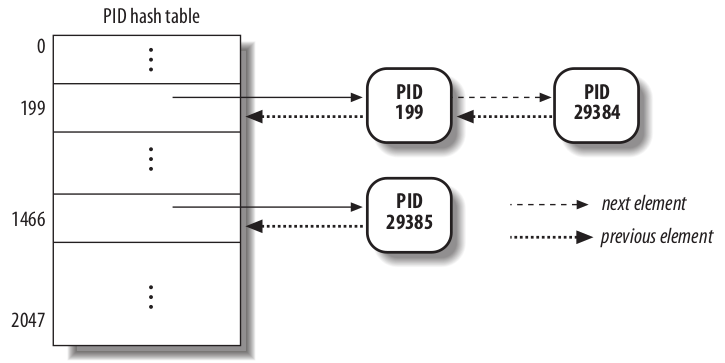
\includegraphics[width=\textwidth]{images/pidhash1}
\caption{Pid hash table, pids 199 and 29384 are both hashed to 199}
\label{img:pidhash1}
\end{figure}

\begin{code}
enum pid_type {
	PIDTYPE_PID,  //process PID
	PIDTYPE_TGID, //thread group leader PID
	PIDTYPE_PGID, //process group leader PID
	PIDTYPE_SID,  //session leader process PID
	PIDTYPE_MAX
};
\end{code}
Code from \verb|include/linux/pid.h|\newline
There are actually four tables, one for each PID type. Each of these tables is an array of \verb|hlist_head|, the head of the chain list, which points to a list of \verb|hlist_node| (see Figure \ref{img:pidhash2}). These  structures are used for non-circular lists. These lists are populated by \verb|struct pid|, and a pointer to this struct is stored inside each process descriptor in the \verb|thread_pid| field. Figure~\ref{img:pidhash2} shows an example for the TGID class that we discussed earlier. PIDs in the chain list are colliding and are different processes, PIDs in the \verb|pid_list| are threads in the same group, where the leftmost thread in the image is the group leader. Despite the name ``\verb|list_head|'' inside the pid structure, such a field points to a circular list, and since it's circular there's really no head structure that points to the first element. %CHECK THIS

\begin{code}
struct pid {
        atomic_t count; // number of references to this PID
	int nr; // PID number
	struct hlist_node pid_chain; // Link to next and previous conflicting entries
	struct list_head pid_list;  // per-PID list
};
\end{code}
Code from \verb|include/linux/pid.h|

\begin{figure}[ht]
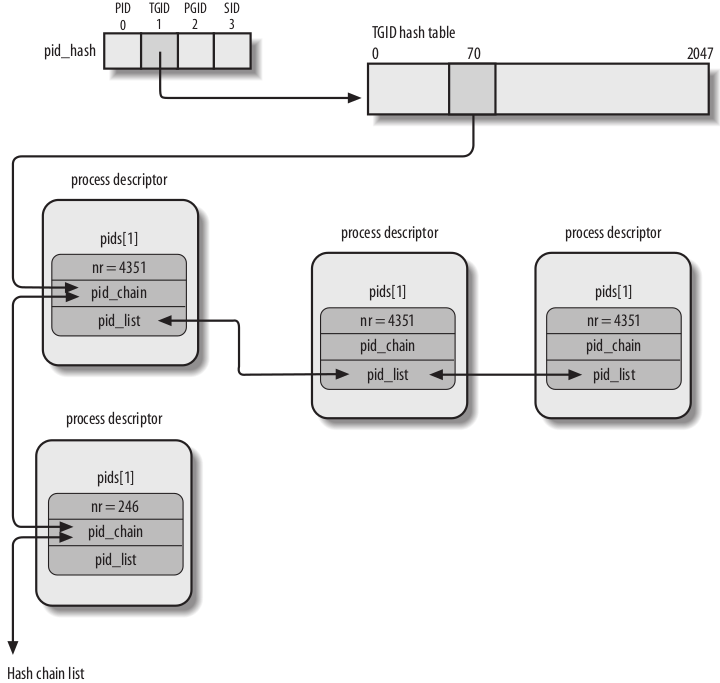
\includegraphics[width=\textwidth]{images/pidhash2}
\caption{Hash table for the TGID pid type}
\label{img:pidhash2}
\end{figure}
The implementation of \verb|struct pid| is slightly different from what was presented, with other nested structures and a different linkage to the hash table. %The way pids are organized is conceptually the same so I presented it like this for semplicity's sake.
In this section, only a small portion of the process descriptor is described. Other fields are illustrated in Section~\ref{chap:implementation}.

%the thread_pid field is a pointer so the struct pid is not actually embedded in the process descriptor, yikes! maybe take a look at this later
%don't use struct pid as an example here for now...

%maybe move this section for later?

\subsection{List implementation}
In a classic circular, the \texttt{struct} of the node contains the data and pointers to the next and previous nodes. This implementation is naive and would lead to have a different structure for each data type, or using a void pointer to your data for no reason. Let's see how lists are used in the kernel.

\begin{figure}[ht]
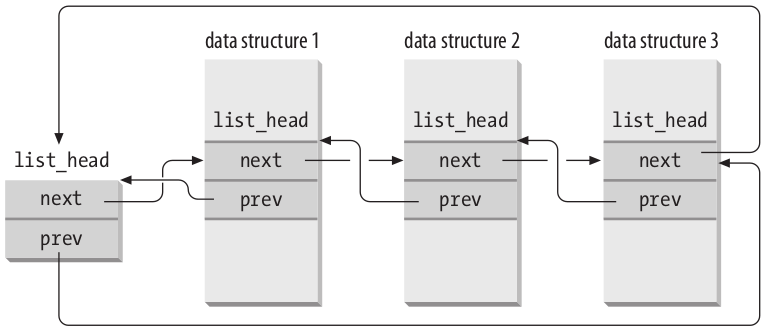
\includegraphics[width=\textwidth]{images/list.png}
\caption{A generic doubly linked circular list}
\label{img:list}
\end{figure}

\begin{code}
struct list_head {
	struct list_head *next, *prev;
};
\end{code}
The data is not contained in the list itself, but in another structure that contains the list node (Figure \ref{img:list}). For example, Linux keeps a big circular list of every \verb|task_struct| in the system: this is done by embedding ``\verb|struct list_head tasks;|'' into \verb|task_struct|. Notice how this is not a pointer to a node: the node is embedded directly into the structure. So how can we get the data we want in the structure without a pointer in the node? The answer is the \verb|container_of()| macro. This macro works with anything, but let's assume that we have a list embedded in the container structure.
\begin{code}
#define container_of(ptr, type, member) ({ \
	void *__mptr = (void *)(ptr); \
	((type *)(__mptr - offsetof(type, member))); })
// An alias that's used everywhere
#define list_entry(ptr, type, member) \
        container_of(ptr, type, member)
\end{code}
Code from \verb|include/linux/kernel.h|\newline
ptr is the pointer to the list node, type is the container struct, member is the field name of the list node in the container struct. We first cast ptr to a void pointer, then we subtract the offset from the beginning of the container struct of the field we want to get. When we allocate a struct, its field are allocated contiguously in virtual memory in the order that we declared them: this means that by moving the pointer backwards from a field by the right amount, we can end up at the beginning of the container structure. This is how we can get the offset of the specified field in any struct:
\begin{code}
#define offsetof(TYPE, MEMBER) ((size_t)&((TYPE *)0)->MEMBER)
\end{code}
Code from \verb|include/linux/stddef.h|\newline
TYPE is the struct we are considering, MEMBER is the name of the field, what it does is:
\begin{enumerate}
    \item Take the address 0, the first in the address space of the process
    \item Cast it to a TYPE pointer 
    \item Dereference the pointer and take the MEMBER field
    \item Take the address of the field and cast it to a size, now it's no longer an address
\end{enumerate}
Essentially, we are pretending that there is the container structure allocated just at the beginning of the address space. This is arguably a bit of a hack, but it's perfectly safe since we are just playing with pointers and never touching actual memory. Indeed, it would be very dangerous to dereference and modify data from a random pointer in memory. This approach has many advantages, such as being able to have multiple lists associated with the same data. \verb|task_struct|, for instance, contains also the \verb|children| and \verb|sibling| lists among many others. This implementation is also very easy to use and it's oblivious about types.

%Mention cooperative multitasking?
\subsection{Scheduling} 
\label{sec:scheduling}
A system with a single CPU can execute only one process at a time. For this reason, a scheduler for processes is needed. Process scheduling consists in choosing which processes should run in what order, essentially deciding how CPU time is shared among processes. To achieve this, there are many scheduling algorithms such as FCFS (\textit{first come first served}), RR (\textit{round robin}), EDF(\textit{earliest deadline first}) and SJF (\textit{shortest job first}). Most of the scheduling policies are \textit{preemptive}, which means that at any time the scheduler can arbitrarily decide to interrupt the currently running task and assign the CPU to another process. The use of preemption implies that processes have assigned \textit{timeslices}: they are periods of time in which the process is allowed to run and after which it will be preempted. 

FCFS, which is the most basic scheduling algorithm, doesn't have preemption nor timeslices: every process runs as much as it wants before voluntarily giving up the CPU to the next task in the queue. Round robin is similar to FCFS because it has a FIFO runqueue; the difference is that it uses a constant timeslice, called \textit{quantum}, assigned to each process: when the quantum expires the process gets preempted and the next task is scheduled.

In a UP (\textit{uniprocessor}) system it is not possible to achieve true parallelism among processes. The only way to do it is to have multiple processors that share a common bus and the central memory: this is known as SMP (\textit{symmetric multiprocessing}). A single processor can also have multiple cores, but each one is treated as a separate processor, so the SMP architecture applies to cores as well. Even on SMP systems, which represent most systems today, there often are more processes than cores. Hence, scheduling is necessary for each processor/core. There are also new problems that arise in SMP, such as \textit{load balancing}: the problem of balancing processes between CPUs so that no CPU goes idle or has an unfair amount of workload. This kind of related problems must also be taken into account by the scheduler.

Every job carried out by the scheduler will eventually lead to a process switch on a given CPU. The kernel has a mechanism to suspend the execution of a process, save its status, and resume another process. This procedure is called \textit{context switch}. Each process has an \textit{execution context}, which includes everything needed for a task to execute, from its stack to the code. While every process can have its own process descriptor, the registers on the CPU must be shared between every process in the system. Every value in any register that a process is using is a subset of the execution context and it's called the \textit{hardware context}. At every context switch the hardware context must be saved and restored, respectively, for the old and the new process. The content of the registers are saved in part in the process descriptor of the preempted process, and in part on its kernel stack.

The routine that performs a context switch is called --- not surprisingly --- \verb|context_switch()|, and it is called only in one well-defined point in the kernel: inside the \verb|schedule()| routine, which triggers the scheduler and chooses the next task to schedule. \verb|context_switch()| (as we will see the code later) basically switches the address spaces of the two processes and then calls \verb|__switch_to()|. This last function operates on registers and kernel stacks, so it's one of the most architecture dependent in the whole kernel. This is why, like many other similar routines, there is one version for each architecture supported by Linux in the \verb|arch| folder. Next, the x86 version of the context switch is described.
%I don't want to go into assembly land and stick to C, so we'll give a high level view of the procedure on x86, though it's important to know some of the registers in the x86 architecture.

There are 6 \textit{segmentation registers} that hold \textit{segment selector}, basically the starting address of memory segments in the process address space.
\begin{itemize}
    \item \verb|cs| \textit{Code segment}, this points to the segment containing instructions of the loaded program, also known as the \verb|.text| section. We mentioned in section \ref{sec:general} that this register also holds 2 bits that describe the current privilege level of the CPU.
    \item \verb|ss| \textit{Stack segment}, points to the segment containing the stack of execution.
    \item \verb|ds| \textit{Data segment}, points to the segment containing global variables and constants, also known as the \verb|.data| section.
\end{itemize}
The other 3, \verb|es|, \verb|fs| and \verb|gs| are general purpose are don't hold a specific address. There are also general purpose data registers that hold data used in operations (\verb|ax|, \verb|bx|, \verb|cx|, \verb|dx|) and pointer registers, that hold offsets:
\begin{itemize}
    \item \verb|ip| \textit{Instruction pointer}, offset to the next instruction. If added to \verb|cs| will be the address of the next instruction to fetch (\verb|cs:ip|).
    \item \verb|sp| \textit{Stack pointer}, offset to the top of stack. If added to \verb|ss| will be the address of the top of stack (\verb|ss:sp|).
    \item \verb|bp| \textit{Base pointer}, offset to subroutine parameters on the stack (\verb|ss:bp|).
\end{itemize}
Let's now see which part of the process descriptor is involved in context switching.
\begin{code}
struct task_struct {
    // ...
    /* CPU-specific state of this task: */
    struct thread_struct    thread;
};
\end{code}
\begin{code}
struct thread_struct {
#ifdef CONFIG_X86_32
    unsigned long	sp0;
#endif
    unsigned long	sp;
#ifdef CONFIG_X86_32
    unsigned long	sysenter_cs;
#else
    unsigned short	es;
    unsigned short	ds;
    unsigned short	fsindex;
    unsigned short        gsindex;
#endif
    // ...
    /* Floating point and extended processor state */
    struct fpu      fpu;
};
\end{code}
This struct is obviously very architecture dependent, its purpose is to save the hardware context before the context switch. You can see that even if it's specific to x86 it can still change depending on 32 or 64-bitness. You can also notice that only a small part of the hardware context gets saved in the process descriptor: the kernel stack pointer, general purpose segmentation registers, data segment and the floating point registers. In older versions of the kernel most of the registers were stored here.
Let's see in detail what happens when the kernel switches from process A to process B. There are actually two different mechanisms in this procedure: the entry/exit mechanism (user/kernel stack switch) and the context switch.
\begin{enumerate}
    \item Process A enters kernel mode, so it will switch from its user stack to its kernel stack, in other words: it saves its \textbf{user} hardware context in the kernel stack. It does so by pushing its \textbf{user mode} stack (\verb|ss:sp|), instruction pointer (\verb|cs:ip|) and data registers onto the kernel stack, then all CPU registers are switched to use the kernel stack.
    \item When in kernel context, process A invokes \verb|schedule()| which will eventually do \verb|context_switch()|.
    \item Process A saves its hardware context: 
    \begin{enumerate}
        \item It pushes most of its register values onto the kernel stack by a series of \verb|mov| assembly operations.
        \item It saves the value of the stack pointer (which is pointing to the \textbf{kernel} stack) into its \verb|task_struct->thread.sp|.
        \item Other registers such as the floating point registers are saved in the \verb|thread| field of \verb|task_struct|.
    \end{enumerate}
    \item Process A loads a previously saved stack pointer from process B's\\ \verb|task_struct->thread.sp|, also loads the other saved registers
    \item Address spaces are switched.
    \item Using the loaded stack pointer, process B moves its previously saved registers from its kernel stack into the registers. This is done by a series of \verb|pop [register]| assembly operations. Process B's state is now completely restored.
    \item process B exits kernel mode and restores its \textbf{user} context. This is accomplished by loading previously saved registers from the kernel stack: its \textbf{user mode} stack (\verb|ss:sp|), instruction pointer (\verb|cs:ip|) and data registers. Process B is now in user context.
\end{enumerate} %checka tutto ciò usando cesati TODO

To understand scheduling mechanisms in the next sections it's important to highlight something in step 2, when the scheduler gets called by a process running in kernel mode. It may be intuitive to think of the scheduler as some kernel thread that is permanently running in kernel mode, but that is not the case. \textbf{The scheduler does not run as a separate thread, it always runs in the context of the current thread.} This means that any process in the system that goes from/to kernel mode can potentially execute the scheduler himself, using its own kernel stack. What exactly can trigger the scheduler is something that we'll see in detail in section \ref{chap:implementation}. The simplest case is when a process voluntarily gives up the CPU by going into a sleep state, in which case it subsequently executes \verb|schedule()| in kernel mode (it would have switched already to kernel mode when sleeping). %CHECK THIS %user preemption and kernel preemption
Another thing to highlight is how the user hardware context has nothing to do with context switch, this is because it always gets saved/restored on the kernel stack when entering/leaving the kernel. An implication of this fact is that context switches always happens in kernel mode, which is expected since it's a core system task.

It's important to understand that a context switch generates significant overhead and, in fact, most of the scheduling overhead comes from context switching. It is caused by the need to switch address spaces and by the fact that context switching is not cache friendly. This is the reason why a context switch between threads (LWP) is almost inexpensive compared to context switching different processes: step 5 in the procedure is skipped because threads share an address space, so there is no need to switch it (again, this is why they are \textbf{lightweight} processes).
%TODO aggiungi cache e controlla

\subsection{Tasks lifetime}
\label{sec:task_lifetime}
Tasks have a life cycle: a new child process task is created every time a task uses fork-like system calls. As shown in Section~\ref{sec:proc_threads}, once a process is created some resources are inherited from the father, depending on the \verb|clone()| flags, while \verb|fork()| will duplicate the calling process. There are some resources that will always be inherited and there is no reason to duplicate, such as the executable object code (the \verb|.text| memory segment in Linux). The new process will be in the runnable state and ready to be scheduled. When the process needs to wait for a particular resource, it goes into a sleep state; it will then become runnable again when the resource is available, or after a predefined time when the syscall \verb|sleep()| is used. A process can also go from running to runnable: this happens if the process is preempted or if it gives up the CPU voluntarily. This last case happens, for instance, if the process needs to do I/O operations for which it doesn't need the CPU. This way no processor time is wasted and another task is scheduled.

A process terminates by executing \verb|exit()| or when it receives  a signal (including \verb|SIGHUP|, \verb|SIGINT|, \verb|SIGKILL|, \verb|SIGTERM|, and others) from other processes which have the privileges to do so. Upon exit, its \textit{exit state} will initially be set to the \textit{zombie} state. A zombie process is a process that terminated, but its process descriptor and entry in the pid hash table are still present in memory and accessible (for example, by \verb|ps -aux|). Tasks' resources are not deallocated immediately because the parent process may want to access some of this information, most likely the \textit{exit status}, or may want to synchronize with the child process termination via \texttt{wait()} ot \texttt{waitpid()}. This is actually a relevant resource leak because \verb|task_struct| is almost 2KB in size. Hence,  if there are many zombie preocesses then a big portion of memory is simply wasted until the parent process executes a \texttt{wait()}/\texttt{waitpid()}. More in details, a \verb|task_struct| plus its kernel stack consumes around 10KB of low kernel memory, that is \verb|THREAD_SIZE + sizeof(struct task_struct)|, assuming that kernel stacks are 8KB in size (\verb|thread_info| and pidhash entry are too small to be relevant).

After terminating and sending a signal to the parent, a task will remain zombie until its parent performs a \verb|wait()|, upon which the parent gets information about the terminated child. Subsequently, \verb|release_task()| is executed and the last data structures from the descriptor get detached. \verb|detach_pid()| is called twice to clear the entry in both the \verb|PID| and \verb|TGID| hash tables, then \verb|task_struct| is finally deallocated. Zombie processes are impossible to kill externally: they can't receive signals as they no longer exists, so a wait by the parent is the only way to clean the memory occupied by the zombie data structure. Suppose that the parent of a zombie process exits without waiting: the child will be an orphan process so it will be become a child of \verb|init|. Luckily, the ancestor process (\verb|init|) has a routine that waits periodically to reap possible zombie processes; so the child process will simply be waited by \verb|init| and get cleared. This mechanism ensures that memory won't be cluttered by zombies and leaves the pid table in a consistent state.
% esempio del comando nella shell figlio del processo della shell con execve?

States and exit states of a process are defined in \verb|include/linux/sched.h| as following.
\begin{code}
/* Used in tsk->state: */
#define TASK_RUNNING    0x0000
#define TASK_INTERRUPTIBLE  0x0001
#define TASK_UNINTERRUPTIBLE    0x0002
#define __TASK_STOPPED			0x0004
#define __TASK_TRACED			0x0008
/* Used in tsk->exit_state: */
#define EXIT_DEAD   0x0010
#define EXIT_ZOMBIE 0x0020
#define EXIT_TRACE  (EXIT_ZOMBIE | EXIT_DEAD)
\end{code}
\begin{itemize}
\item \verb|TASK_RUNNING| is either a process that is ready to be run
  (in which case it's more like ``runnable'') or that is actually
  running.

\item   \verb|TASK_INTERRUPTIBLE| and \verb|TASK_UNINTERRUPTIBLE| are both
  states in which a task is sleeping, waiting for some condition to
  be true. The former allows a process to be woken up by signals, the
  latter does not: an uninterruptible task will ignore any signal and
  will only wake up on his condition. This distinction is the reason
  why, as we will see later, the routine that wakes up tasks is called
  \verb|try_to_wake_up()|. 
\item \verb|__TASK_TRACED| means that another process is tracing this
  one, usually a debugger such as \verb|ftrace| (as explained in
  Section~\ref{chap:ftrace}).
\item A task in \verb|__TASK_STOPPED| is not running and cannot be
  scheduled: this happens upon stop signals or any signal from a
  tracing process.
\end{itemize}

The values associated to these states are defined like this so that they can be used for bitmasks, which is the standard way to handle flags. Each flag is a power of 2 (in hexadecimal) so flags can be combined with bitwise operator \verb&|& or be tested with \verb|&|. For example, checking if a task is sleeping can be easily done like this: 

\begin{code}
if(tsk->state & (TASK_INTERRUPTIBLE | TASK_UNINTERRUPTIBLE))
    printk("task %d is waiting for something", tsk->pid); 
\end{code}

\begin{figure}[ht]
  \centering
  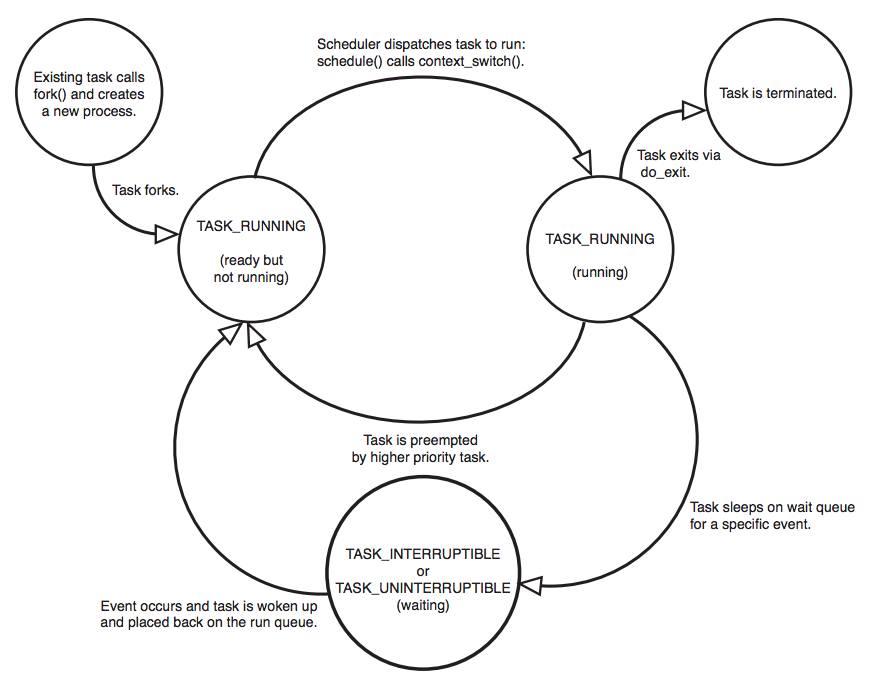
\includegraphics[width=0.75\textwidth]{process_life} %add try_to_wake_up in the image or make a new one
  \caption{State machine of task states}
  \label{img:process_life}
\end{figure}
